%set the master document for easy compilation
%!TEX root = ../D3_5_3.tex

The system architecture of the openETCS OBU is adapted from the system structure defined in ERA Subset-026 Chapter 2.5 \cite{subset-026}. Figure \ref{f:architecture_srs} shows which parts of the reference architecture are in the scope of the openETCS OBU model. Note that also specific parts of the ETCS trackside (e.g.~Eurobalise and RBC blocks) have been modeled to have an integrated test environment, c.f.~dashed blue line in Figure~\ref{f:architecture_srs}.

\begin{figure}
\centering
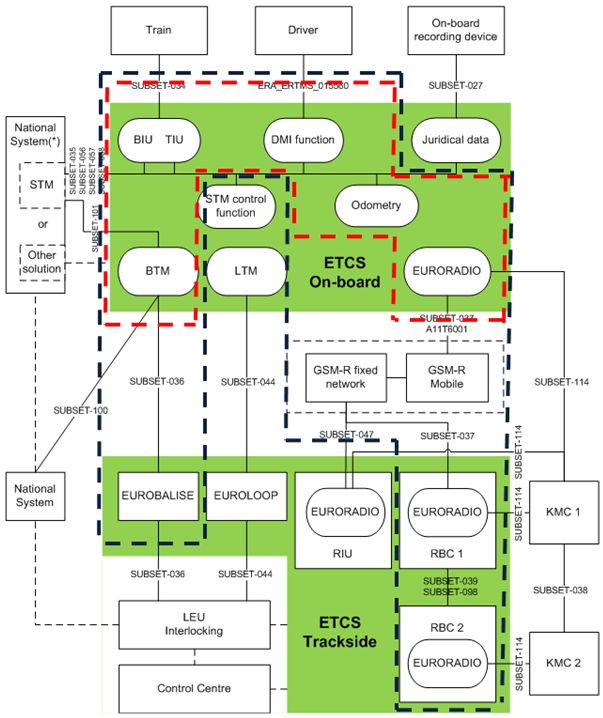
\includegraphics[width=.7\textwidth]{images/ArchitectureSRS}
\caption[Scope of openETCS OBU model system according to ERA TSI Chapter 2.5.]{Scope of openETCS OBU model system according to ERA TSI Chapter 2.5. Functional blocks in the scope of openETCS have been marked by the dashed blue line. The dashed red line shows the OBU blocks in the scope of openETCS.}
\label{f:architecture_srs}
\end{figure}


\section{Top Level Architecture and External Interfaces}

Figure~\ref{f:top_level} shows the top level architecture with external interfaces E1, E2,$\ldots$, E9.
\begin{figure}
\centering
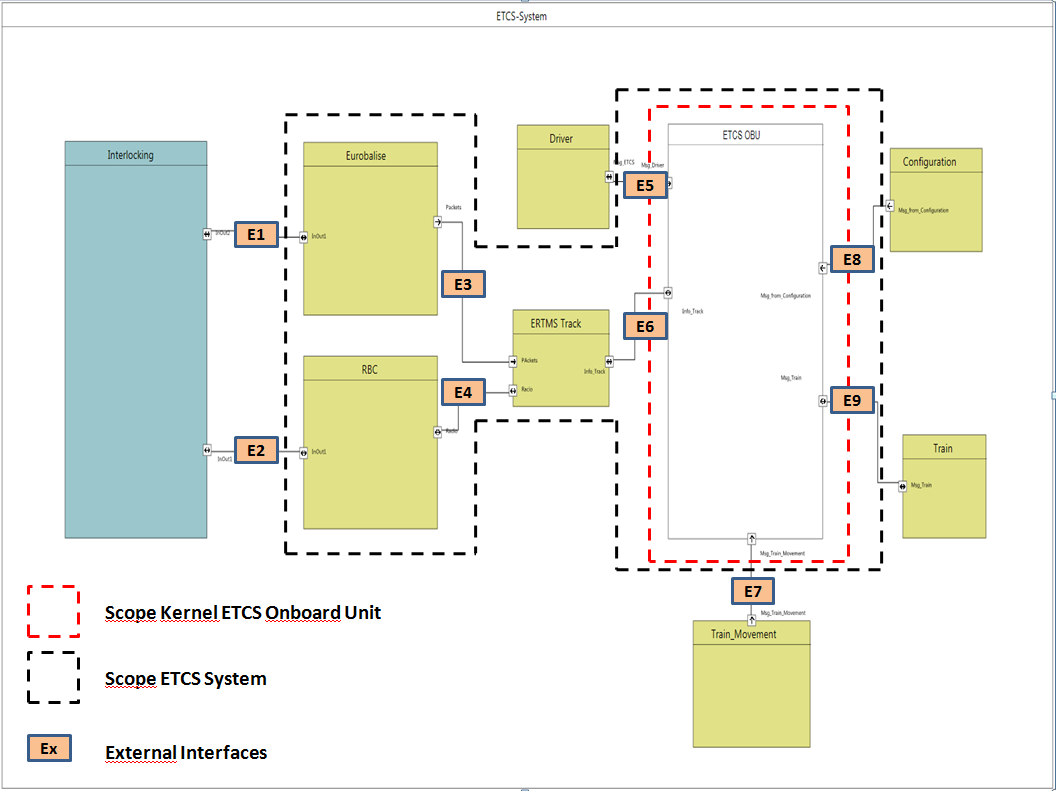
\includegraphics[width=\textwidth]{top_level_architecture.png}
\caption{Top level architecture with external interfaces.}
\label{f:top_level}
\end{figure}
The external interfaces are used for the communication between the openETCS OBU (dashed red line) and systems out of the scope of the openETCS project and the ETCS Onboard Unit System.\todo[fancyline]{paragrapoh has to be checked and extended to be more clear} In the following we give  brief overview of the interfaces:
\begin{description}
\item[E1:] In- and out flow between the Interlocking and the Eurobalise. Only relevant for controlled Eurobalises.

\item[E2:] In- and out flow between the Interlocking and Radio Block Control.
This interface ensures the states or logics directly to the Radio Block Control and the other way back from the train to the interlocking.

\item[E3:] Input flow from the Eurobalise to the Balise Transmission Module or Antenna Unit (BTM) into the ETCS OBU.

\item[E4:] In- and out flow between the Radio Block Control and the Euroradio modul into the ETCS OBU. This interface is not active in ETCS levels 0 and 1 since there is no ETCS radio interaction between track and train in these levels.

\item[E5:] This interface is used for the interaction between the driver and the display (Driver Machine Interface, DMI), c.f.~Figure \ref{DMI Interfaces}.\todo[fancyline]{check if figure is correct. Do we need this figure anyway? If so, make it more appealing.}
\begin{figure}
\centering
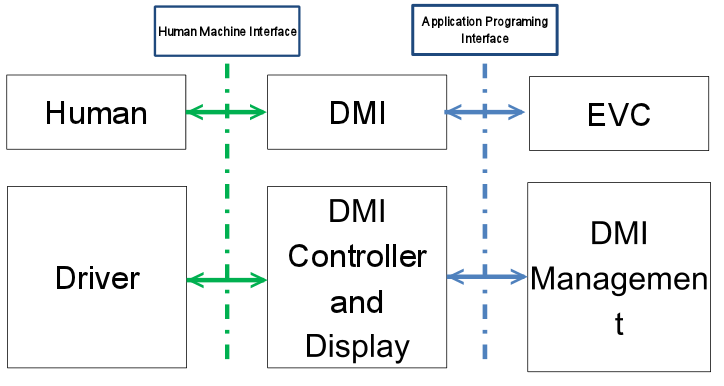
\includegraphics[scale=0.5]{images/DMIinterfaces}
\caption{DMI Interfaces.}
\label{DMI Interfaces}
\end{figure}

\item[E6:] This interface is a compound structure and combines the interfaces E3 and E4.

\item[E7:] Input interface to the odometry subsystem of the ETCS OBU. Used for sending information to the train if there is any movement outside the ETCS System, e.g.~"cold movement".

\item[E8:] Input interface to the ETCS OBU to set configuration data such as fixed values, system values, national values and train configuration.

\item[E9:] In- and Out flow between the ETCS OBU and the train. This interface is used for the interaction between the Train and the ETCS OBU such as brake control, traction control, door control, etc.
\end{description}


\section{Functional breakdown of the ETCS OBU}

Figure \ref{f:ETCS_OBU_decomposition} depicts the functional breakdown of the ETCS OBU block shown in Figure~\ref{f:top_level}.\todo{Figure is incomplete and erroneous... F2 is not connected, F2 exists twice}\todo{Should this block be described using the new component description template? Section needs to be completed} The internal interfaces
\begin{figure}
\centering
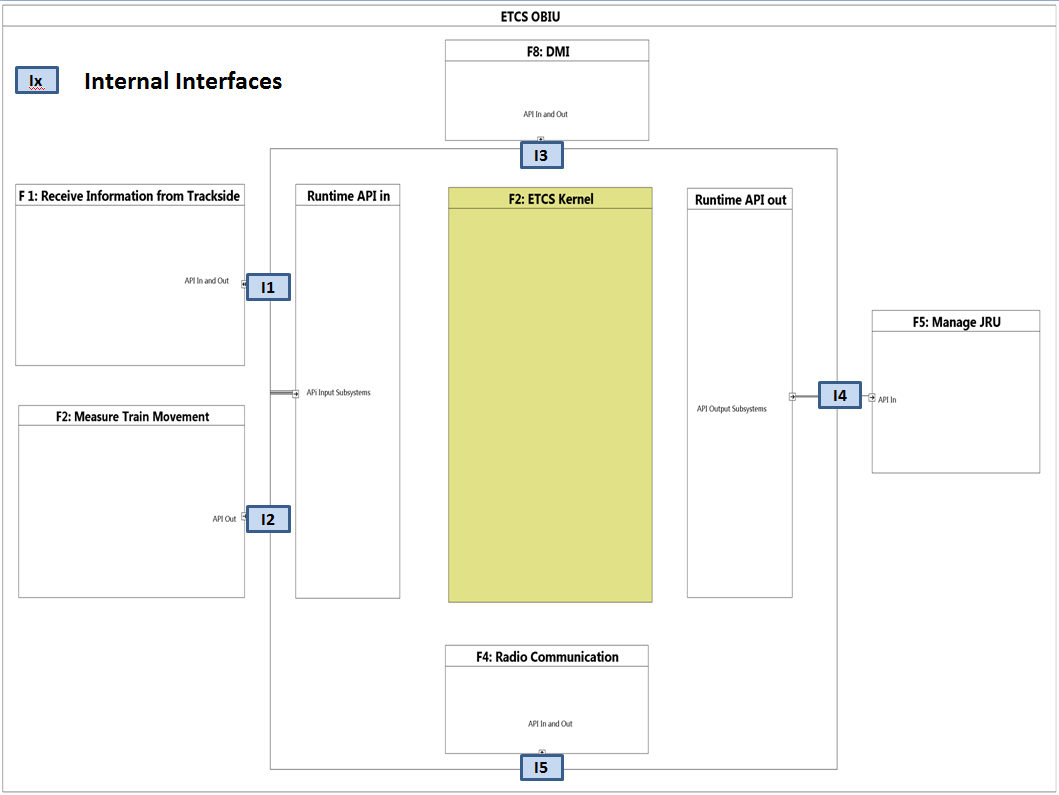
\includegraphics[width=\textwidth]{images/2ndlevelarchitecture}
\caption{2nd level system architecture view.}
\label{f:ETCS_OBU_decomposition}
\end{figure}
\begin{description}
\item[I1:] In flow from the Balise Transmission Module (BTM or Antenna) to the "F2 ETCS Kernel" trough Runtime API in. Transmitted data are information from the Eurobalise.

\item[I2:] In flow from the Odometrie (ODO) to the "F2 ETCS Kernel" trough Runtime API in. Transmitted data are information from the movement of the train.

\item[I3:] In- and Out flow between the DMI Controller and the "F2 ETCS Kernel" trough Runtime API in and out. Transmitted data are information of driver action and display. See description in figure of "External Interface E5".

\item[I4:] Out flow from "F2 ETCS Kernel" to the JRU manager trough Runtime API out. Transmitted data are all necessary information for a juridical recorder unit "black box".

\item[I5:] In- and Out flow between the Euroradio and "F2 ETCS Kernel" trough Runtime API in and out. Transmitted data are radio track information (RBC) and information to the track (RBC). 
\end{description}






